\chapter{Fórmula de Clark--Ocone y cobertura}\label{cap:clark-ocone}

\begin{teorema}[Clark--Ocone, \guia{Teorema 8.9}]
Si $F\in\Dom$ es $\F_T$-medible,
\[
  F=\E[F]+\int_0^T\E[\D_tF\mid\F_t]\dd W_t.
\]
\end{teorema}

\begin{ejemplo}
$F=W_T^3$: $\D_tF=3W_T^2$ y $\E[3W_T^2\mid\F_t]=3(W_t^2+T-t)$.
\end{ejemplo}

\section{Cobertura en Black--Scholes}
Bajo $\Q$, $\dd S_t=rS_t\dd t+\sigma S_t\dd W_t$ y $\tilde S_t=e^{-rt}S_t$ cumple
$\dd\tilde S_t=\sigma\tilde S_t\dd W_t$. Para el pago descontado
$F=e^{-rT}\Phi(S_T)$, Clark--Ocone da
\[
  F=\E_\Q[F]+\int_0^T\phi_t\dd W_t=\E_\Q[F]+\int_0^T\Delta_t\dd\tilde S_t,\qquad
  \Delta_t=\frac{\phi_t}{\sigma\tilde S_t}.
\]
Para la call, $\D_tF=e^{-rT}\ind_{\{S_T>K\}}\sigma S_T$ y
$\E[\D_tF\mid\F_t]=\sigma\tilde S_t\,N(d_1(t))$: se recupera la delta de
Black--Scholes, $\Delta_t=N(d_1(t))$ \guia{Ejemplo 13.2}. Para la digital
\guia{Ejemplo 13.3}, $\Delta_t=e^{-r(T-t)}\varphi(d_2)/(\sigma S_t\sqrt{T-t})$ para $t<T$
(\codigo{clark\_ocone.integrand\_digital}). La ventaja del enfoque es que se generaliza a
pagos dependientes de la trayectoria y a modelos sin EDP explícita
\cite{oconekaratzas1991,dinunno2009}.

\begin{figure}[h]
  \centering
  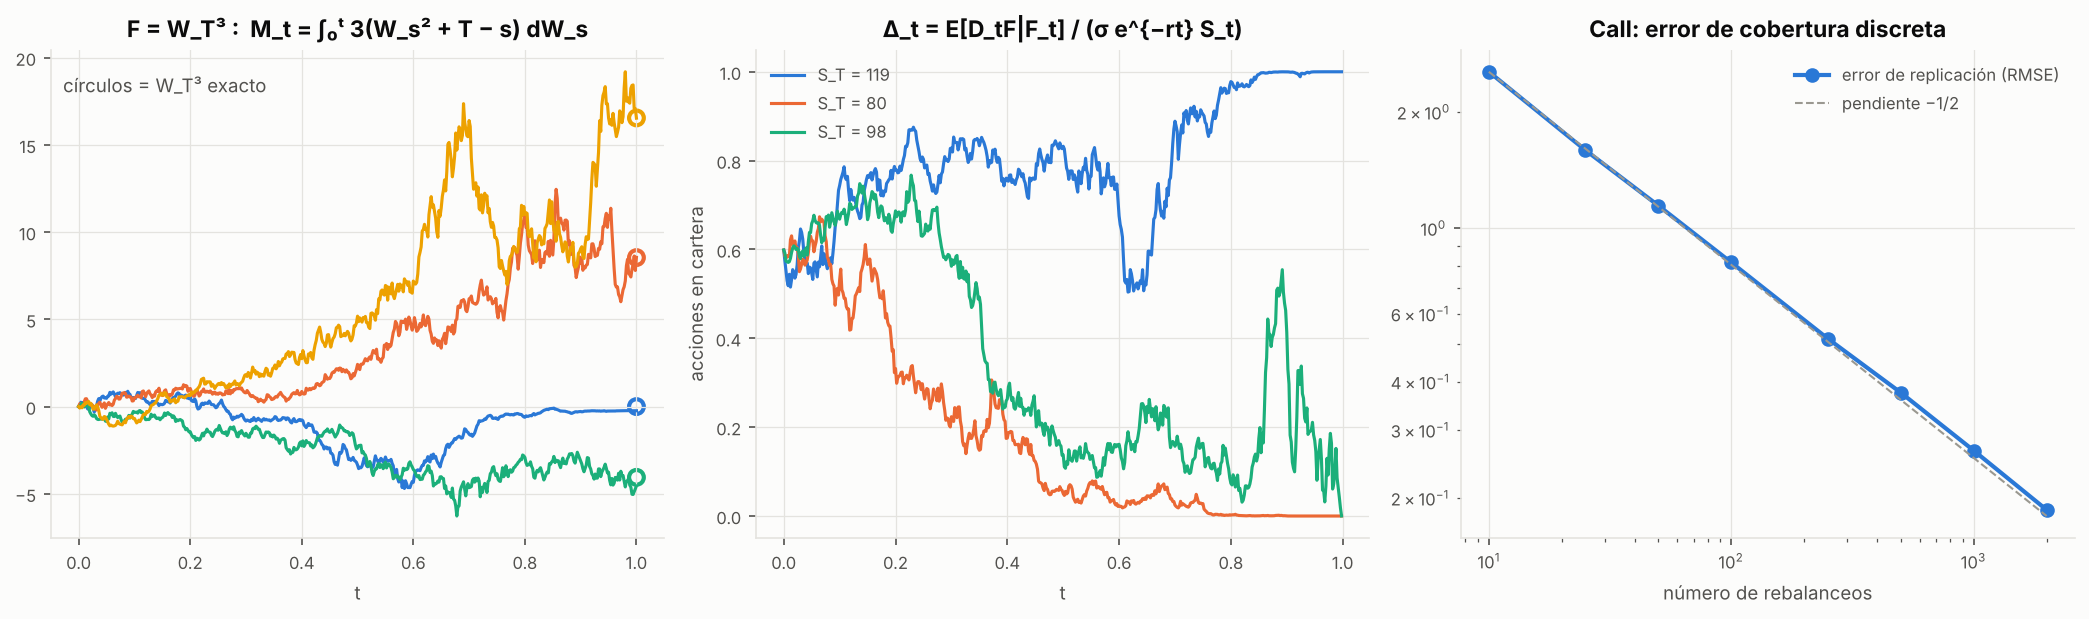
\includegraphics[width=\linewidth]{04_clark_ocone_cobertura}
  \caption{Reconstrucción de $W_T^3$, deltas de cobertura y error de replicación
  discreto $\propto n^{-1/2}$ (\codigo{examples/04\_clark\_ocone\_cobertura.py}).}
\end{figure}
